\chapter{Benchmarking}
\label{chap:benchmarking}

This chapter operationalizes the benchmark design principles derived from Chapter~\ref{chap:state-of-the-art}. In particular, it aims to address the evaluation pathologies highlighted by \textcite{liu2024elephant} (Section~\ref{sec:systemic-benchmarking-challenges}) while implementing the domain-specific requirements summarized in Section~\ref{sec:synthesis-related-work}.

Concretely, the benchmark is constructed to (i) provide clean baseline periods that models can train on or condition on, (ii) represent multivariate contextual point anomalies in the sense of covariate-conditioned detection on consumption targets, and (iii) test seasonal translation by evaluating models under controlled seasonal distance between baseline and evaluation windows.

\section{Benchmark Design and Dataset Generation}
\label{sec:benchmark-design}

To evaluate detection robustness under realistic non-stationary building dynamics, a synthetic benchmark dataset was generated with the \ac{BOPTEST}\parencite{Blum03092021}. The benchmark isolates physical building behavior from telemetry artifacts, providing a controlled yet realistic evaluation environment.

A full year of 15-minute resolution data was produced from the \textit{Multizone Office Complex Air} test case\parencite{BOPTESTMultizoneOfficeComplexAir}, which represents a large office building with coupled thermal zones, air-handling units, and realistic occupancy schedules. This annual baseline captures seasonal dynamics and supports out-of-season generalization tests while avoiding sensor dropouts or undocumented control overrides.

\section{Feature and Target Definition}
\label{sec:benchmark-features}

The exported telemetry was decomposed into contextual drivers and consumption targets. Control-loop variables were explicitly excluded to prevent fault leakage into the feature space, ensuring that anomalies remain detectable through residual behavior rather than direct control-state exposure.

Contextual features include weather variables, occupancy counts, calendar indicators, and cyclical encodings of diurnal and annual patterns. Seventeen electrical meters were treated as targets, spanning the aggregate main meter alongside critical \ac{HVAC}, pumping, and lighting subsystems to support both financial attribution and hierarchical diagnostics.

\begin{figure}[htbp]
	\centering
	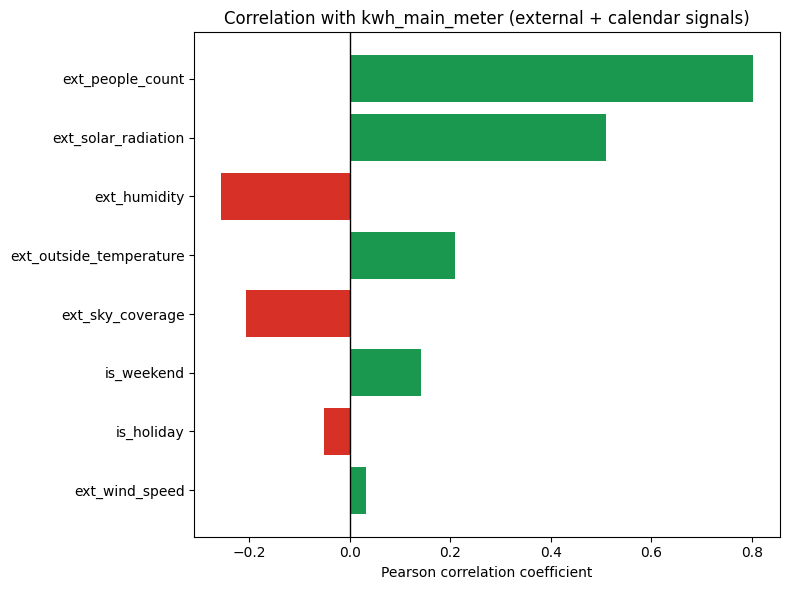
\includegraphics[width=0.9\textwidth]{images/feature-improtance.png}
	\caption{Empirical Pearson correlation of contextual and external drivers with the main electricity meter over the created dataset from \ac{BOPTEST}.}
	\label{fig:feature-importance}
\end{figure}

\section{Data Segmentation and Anomaly Injection}
\label{sec:benchmark-anomalies}

The annual baseline was segmented into multiple training--evaluation regimes to assess sample efficiency and seasonal generalization, including six-month, three-month, and two-week windows. Injected anomalies were constrained to remain below 5\% of total points to preserve realistic anomaly prevalence on the main meter and sub-meters (see Section~\ref{rw:unrealistic-anomaly-ratios}).

Synthetic perturbations emulate realistic operational, control, and contextual fault classes such as sustained drifts, extended deviations, off-hours activity, pattern shifts, and localized spikes. Each anomaly is labeled with onset, duration, and magnitude to support fine-grained evaluation of detection latency, persistence coverage, and financial attribution.

\begin{figure}[htbp]
	\centering
	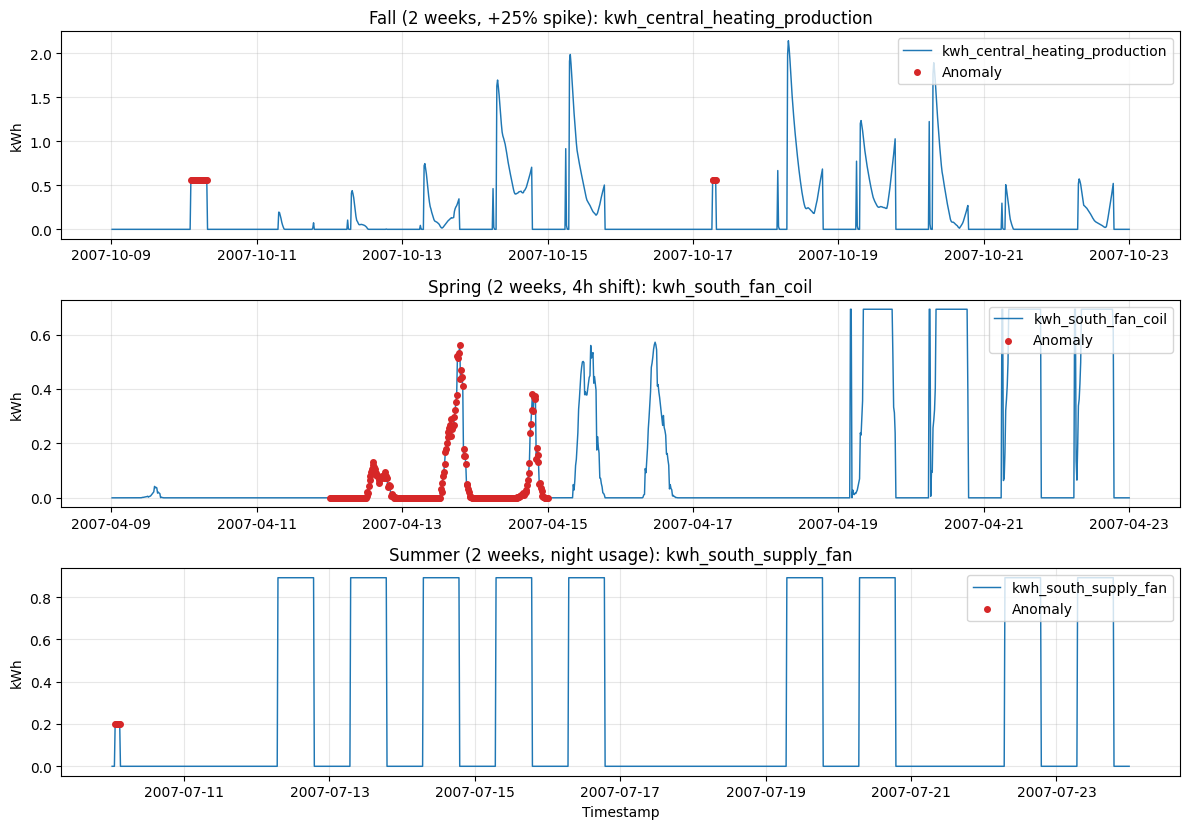
\includegraphics[width=0.92\textwidth]{images/anomaly-dataset-examples.png}
	\caption{Representative sub-meter excerpts from the curated benchmark slices (fall spike, spring pattern shift, summer off-hours). Red markers indicate anomaly windows where the targeted device deviates from its baseline regime.}
	\label{fig:anomaly-dataset-examples}
\end{figure}


\section{Evaluation Constraints and Benchmark Limitations}
\label{sec:benchmark-limitations}

While the BOPTEST-based benchmark enables controlled and reproducible evaluation,
several constraints affect the interpretation and comparability of the resulting
metrics.

\subsection{Training Stability and Coverage Bias}

Several evaluated architectures require extensive per-meter hyperparameter tuning.
\ac{MDN}s in particular exhibit high sensitivity to initialization
and regularization, leading to unstable convergence on subsets of meters.

As a consequence, benchmark coverage differs substantially between methods. Aggregate
scores for unstable models are computed over reduced subsets of meters, introducing
implicit coverage bias. Reported performance therefore reflects both detection accuracy
and training robustness under limited tuning budgets.

\subsection{Comparability Across Model Classes}

Trainable models are trained on season-specific clean baseline windows and are
evaluated on held-out segments drawn from the same baseline regime, into which
synthetic anomalies are injected. Anomaly detection therefore operates relative to a
consistent normative reference distribution.

\ac{TSFM} models, in contrast, cannot be conditioned on the evaluation window
itself. They must infer normative behavior exclusively from preceding historical
context, which may belong to a different seasonal or operational regime. As a result,
detection is performed relative to a shifted baseline distribution rather than the true
local operating regime of the evaluation window. This induces a structural evaluation
asymmetry that becomes most pronounced in short-window and seasonal translation
experiments.

The season-matched three-month baseline configuration provides the closest
approximation of comparable operating conditions. In this configuration, Chronos-2
can condition on the complete baseline history within its maximum context length,
thereby minimizing structural disadvantages relative to trainable models.


\subsection{Interpretation Scope}

Benchmark metrics should therefore be interpreted as indicators of practical
deployability and robustness under realistic engineering constraints rather than as
absolute measures of algorithmic superiority. Emphasis is placed on persistence
tracking, qualitative behavior, and economic interpretability rather than raw
aggregate scores alone.

\section{Comparative Model Performance and Structural Evaluation}
\label{sec:comparative-model-performance}

A total of up to 16{,}979 benchmark runs per model were executed across all dataset
slices. Classical \ac{CNN} baselines adapted from the \ac{TSB-AD} benchmark perform poorly on
building-energy telemetry despite strong multivariate results in generic \ac{TSAD}
benchmarks, confirming that autoregressive input windows destabilize \ac{TSAD}.

A \ac{CNN} Feature-Only architecture that relies solely on exogenous contextual drivers
achieves markedly higher detection scores, indicating that contextual baselines
provide superior normative representations for building-scale telemetry.

Figure~\ref{fig:mdn-dense-cnn-baseline-comparison} summarizes the aggregate comparison across benchmark slices, while Figure~\ref{fig:mdn-dense-cnn-baseline-comparison-mainmeter} isolates the building main meter to highlight the effect of stochastic output modeling under stable training conditions.

\begin{figure}[htbp]
	\centering
	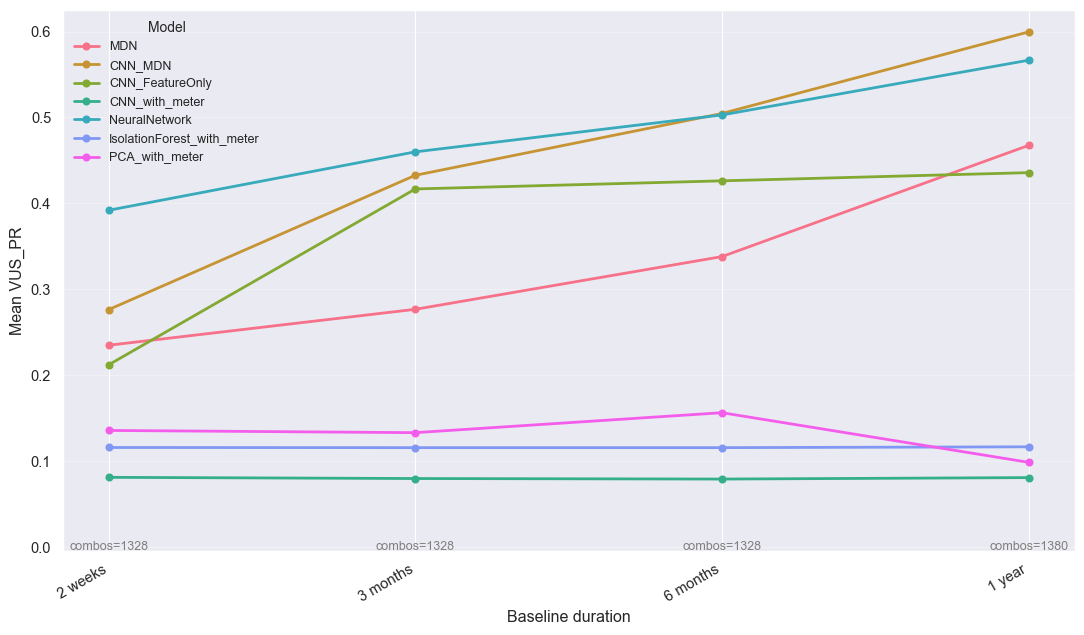
\includegraphics[width=1.0\textwidth]{images/mdn-dense-cnn-baseline-comparison.png}
	\caption{Comparison of neural baselines and mixture-density variants across benchmark slices.}
	\label{fig:mdn-dense-cnn-baseline-comparison}
\end{figure}

\begin{figure}[htbp]
	\centering
	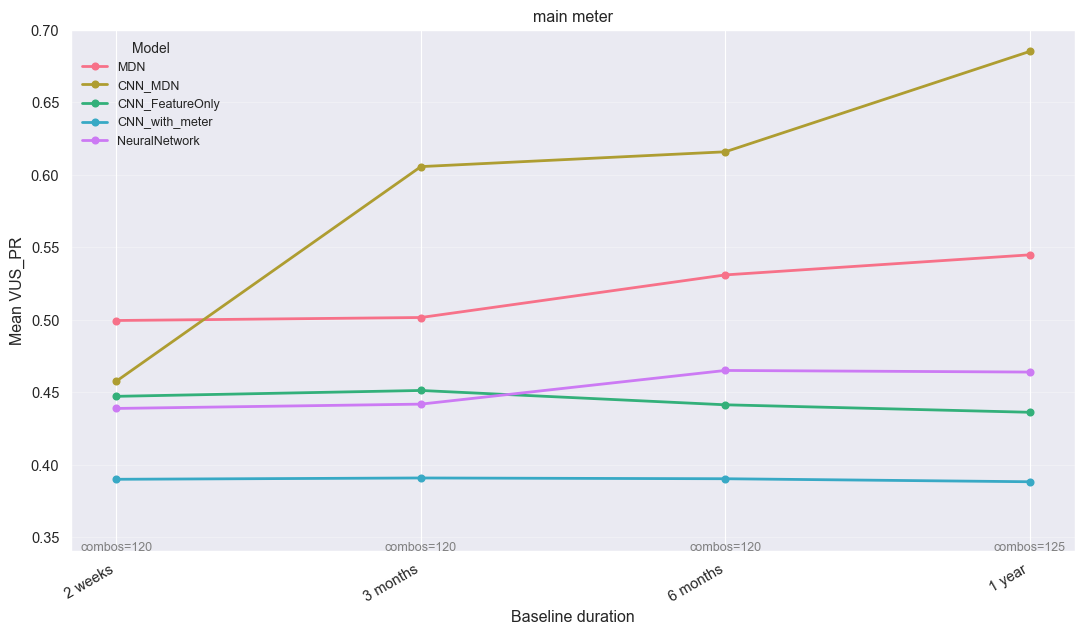
\includegraphics[width=1.0\textwidth]{images/mdn-dense-cnn-baseline-comparison-mainmeter.png}
	\caption{Benchmark comparison on the building main meter, highlighting feature-only and stochastic output effects.}
	\label{fig:mdn-dense-cnn-baseline-comparison-mainmeter}
\end{figure}

\subsection{Stochastic and Hybrid Architectures}
\label{subsec:stochastic-hybrid-architectures}

Pure \ac{MDN}s seem to underperform deterministic contextual models. In
contrast, the hybrid \texttt{CNN\_\allowbreak MDN} delivers the highest \ac{VUS-PR} on
long-horizon baselines, while residual dense networks dominate short-horizon
regimes. Detection accuracy increases monotonically with the amount of baseline
context available for training in almost all models.

\subsection{Training Stability and Classical Baselines}
\label{subsec:training-stability-baselines}

\ac{MDN} layers exhibit sensitivity to initialization and regularization, leading to
coverage gaps across meters. \ac{PCA} and Isolation Forest baselines consistently yield
the lowest performance, confirming that linear and tree-based statistical models fail
to capture the non-linear contextual dependencies present in building-energy
telemetry. The consolidated training history remains available in
Appendix~\ref{app:training-history} (Figure~\ref{fig:training-history-all-meters}).

Importantly, the main meter provides a representative example where \ac{MDN}-based models (including \texttt{CNN\_\allowbreak MDN}) converged stably, which is why Figure~\ref{fig:mdn-dense-cnn-baseline-comparison-mainmeter} is reported separately. In that setting, \ac{MD}-based stochastic output modeling yields a substantially stronger \ac{VUS-PR} than deterministic baselines, suggesting that the weaker aggregate \ac{MDN} scores in Figure~\ref{fig:mdn-dense-cnn-baseline-comparison} are partly a consequence of per-meter instability and reduced coverage rather than an inherent lack of modeling capacity. This limits the strict comparability of aggregated results but still provides evidence for the advantages of probabilistic mixture modeling as discussed in Section~\ref{sec:md-anomaly-scoring}.

\subsection{Season-Matched Three-Month Evaluation}

To minimize seasonal confounding, models were compared under a season-matched
three-month baseline. While \texttt{CNN\_\allowbreak MDN} attains the strongest mean
\ac{VUS-PR}, deterministic neural baselines remain competitive on several anomaly classes.
This configuration is used for the most direct comparison between the foundation model Chronos-2 and trainable baselines, as it minimizes informational asymmetry by aligning the seasonal regime and providing sufficient baseline context.
Chronos-2 performs better than most models, with fine-tuning improving it only minimally in
off-hours detection. PatchTST\parencite{nie2022time} and OmniAnomaly\parencite{su2019robust} underperform, whereas Autoformer\parencite{wu2021autoformer} shows
strong performance on spike-like anomalies.

This comparison is visualized in Figure~\ref{fig:chronos-vs-cnnmdn}.

\begin{figure}[htbp]
	\centering
	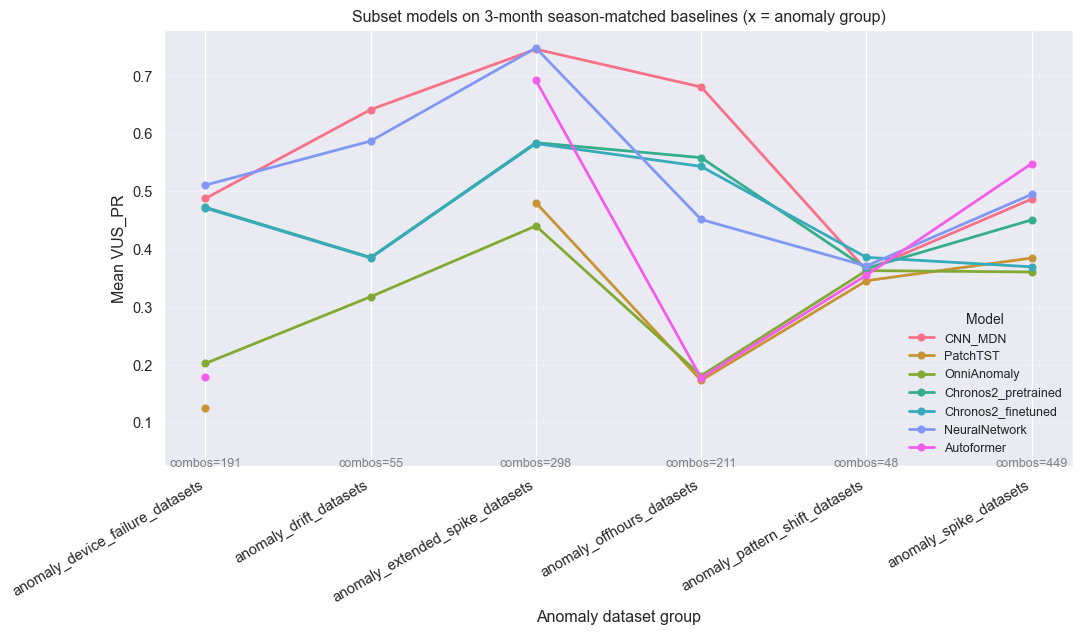
\includegraphics[width=1.0\textwidth]{images/chronos-vs-cnnmdn.png}
	\caption{Chronos-2 vs. \texttt{CNN\_\allowbreak MDN} under season-matched three-month baselines.}
	\label{fig:chronos-vs-cnnmdn}
\end{figure}

\subsection{Seasonal Translation Sensitivity}

Mean \ac{VUS-PR} degrades monotonically as the seasonal distance between training and
evaluation windows increases. The largest performance losses are observed for
\texttt{CNN\_\allowbreak MDN} and OmniAnomaly, while Autoformer and PatchTST remain comparatively
stable across seasonal shifts.

Figure~\ref{fig:seasonal-distance} summarizes this translation sensitivity.

\begin{figure}[htbp]
	\centering
	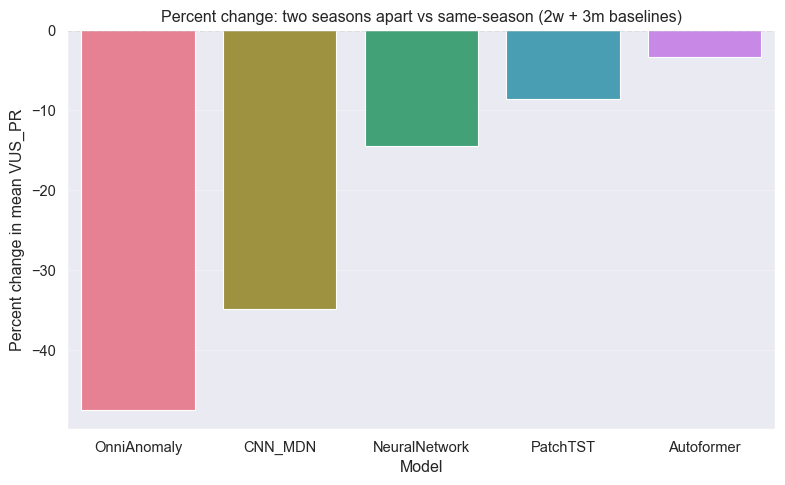
\includegraphics[width=1.0\textwidth]{images/sesonal-distance.png}
	\caption{Seasonal translation sensitivity of mean \ac{VUS-PR} versus seasonal distance.}
	\label{fig:seasonal-distance}
\end{figure}

\subsection{Model Selection Rationale}
\label{sec:model-selection-rationale}

Although \texttt{CNN\_\allowbreak MDN} attains the highest mean \ac{VUS-PR} in most benchmark
configurations, Chronos-2 is selected as the primary deployment model because it best
satisfies the thesis objectives under portfolio-scale constraints. In particular, the
zero-shot, context-conditioned operating mode of \acp{TSFM} directly supports
~\textbf{O\ref{obj:drift-robustness}} by adapting to baseline drift and abrupt
regime changes through recent-context conditioning rather than scheduled per-meter
retraining pipelines. This simultaneously strengthens practical scalability
(~\textbf{O\ref{obj:horizontal-scalability}}) and preserves context-conditioned
normality (~\textbf{O\ref{obj:contextual-fidelity}}).

Trainable baselines require explicit per-meter fitting and repeated retraining to track
non-stationarity, implying fragile orchestration at scale. Persisting anomalies are
prevented from contaminating the adaptive reference by applying Strategy~B from
Section~\ref{sec:inference-time-imputation}, which operationalizes
~\textbf{O\ref{obj:persistence-preservation}} in the deployed pipeline.

While Chronos-2 does not expose an explicit multimodal mixture density, it provides
calibrated, distribution-free quantile bounds (Section~\ref{subsec:quantile-bounds}),
which satisfy ~\textbf{O\ref{obj:distributional-validity}} sufficiently for
deployment. These quantile envelopes enable \ac{QBB} anomaly scoring without
parametric assumptions and avoid the instability and coverage gaps observed for
mixture-density architectures, while remaining competitive in detection accuracy.

